% ===================== PARTE 5: DOS MÁQUINAS, EL MISMO PROGRAMA (diapositivas 52-62) =====================
\parte{Dos máquinas, el mismo programa}{Dos máquinas, el mismo programa:\\i5-10400 frente a Core Ultra 9}
  {El mismo guion, los mismos parámetros y el mismo compilador en las dos. ¿Se mantiene el orden de los algoritmos? ¿Y por qué una CPU el doble de rápida pierde con contención?}{s52}

\begin{frame}{Cómo se comparan las dos máquinas}
  \fuente{codigo/ejecutar\_pruebas.sh; datos de corrección del i5-10400 y del Ultra 9}
  \begin{columns}[T]
    \column{0.56\textwidth}\footnotesize\renewcommand{\arraystretch}{1.18}
    \begin{tabularx}{\linewidth}{@{}>{\leavevmode\color{gris}}p{0.22\linewidth}XX@{}}
      \toprule
      & \textbf{Core i5-10400} & \textbf{Core Ultra 9 285}\\
      \midrule
      Núcleos & 6, con SMT: 12 hilos & 24 (8 P + 16 E), sin SMT\\
      Sistema & WSL2 sobre Windows & Linux nativo\\
      Compilador & g++ 13.3 & g++ 13.3\\
      Programa & \multicolumn{2}{l}{\texttt{bench.cpp}, sin alinear, sin jemalloc}\\
      Rendimiento & \multicolumn{2}{l}{1\,s por punto, 1 pasada; hilos 1, 2, 4, 8, 12 y 18}\\
      Escenarios & \multicolumn{2}{l}{$n = 1$, 10 y \pot{5}; $u = 1$, 10 y 50\,\%}\\
      Latencia & $p = 1$ y $p = 12$ & $p = 1$ y $p = 24$\\
      \bottomrule
    \end{tabularx}
    \column{0.4\textwidth}
    \caja{Mismo guion, mismos parámetros, mismo compilador: la diferencia está en la máquina.}
    \par\medskip
    \aviso{Una sola pasada de 1\,s: solo cuentan las diferencias grandes, de 2\por{} o más, y el orden de los algoritmos. Los paneles $n = 10$ llevan el freno de la compartición falsa (\hyperlink{parte6}{parte 6}) en las dos máquinas.}
  \end{columns}
  \nota{s53}
\end{frame}

\begin{frame}{Core i5-10400: pasada rápida de \texttt{bench.cpp}}
  \fuente{rendimiento.csv del i5-10400; 1 pasada de 1\,s por punto; misma escala vertical que la siguiente diapositiva}
  \centering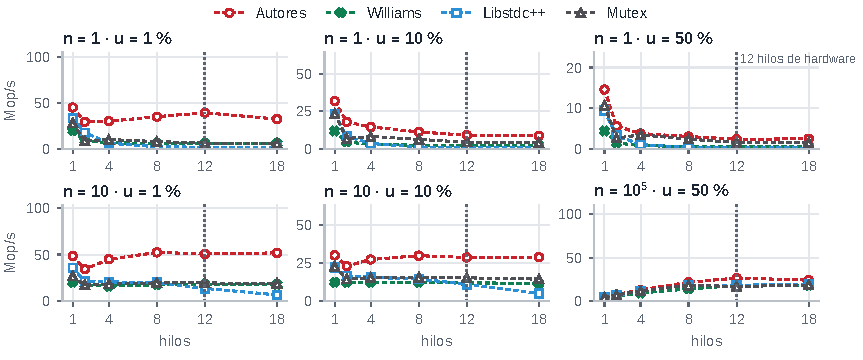
\includegraphics[width=\linewidth]{figuras/s54}
  \nota{s54}
\end{frame}

\begin{frame}{Core Ultra 9 285: el mismo programa, la misma escala}
  \fuente{correccion/rendimiento.csv del Ultra 9; 1 pasada de 1\,s por punto}
  \centering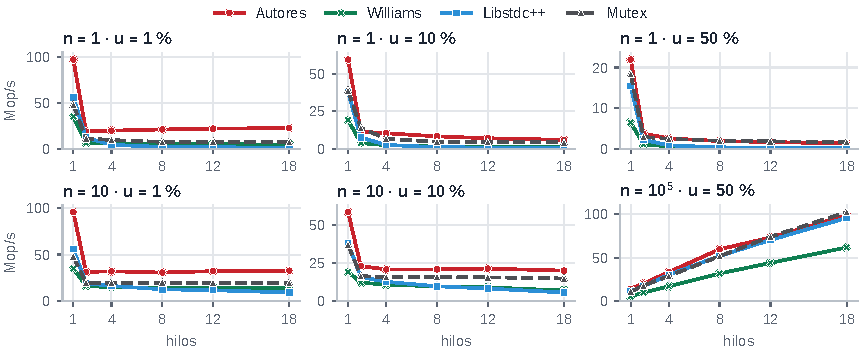
\includegraphics[width=\linewidth]{figuras/s55}
  \nota{s55}
\end{frame}

\begin{frame}{El orden de los algoritmos se mantiene en las dos máquinas}
  \fuente{rendimiento.csv del i5-10400 y del Ultra 9 (correccion), 12 hilos}
  \centering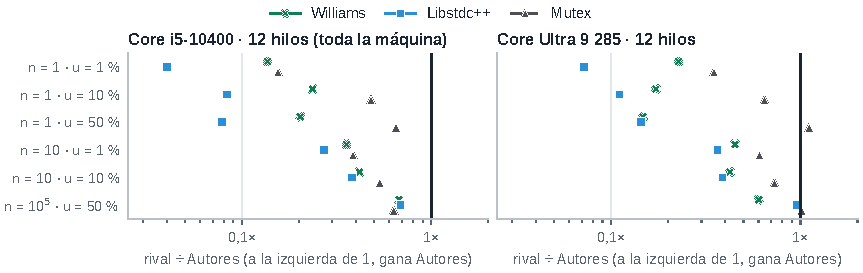
\includegraphics[width=\linewidth]{figuras/s56}
  \vfill\raggedright
  \caja{Con 12 hilos, \textbf{Autores gana a Williams y a Libstdc++ en los 6 escenarios y en las dos máquinas} (en el Ultra 9, con \pot{5} pilas, a Libstdc++ solo por un 4\,\%). La única diferencia es el Mutex con $n = 1$ y $u = 50$\,\%: en el Ultra 9 gana a Autores; en el i5, no.}
  \nota{s56}
\end{frame}

\begin{frame}{Con un hilo el Ultra 9 es el doble de rápido; con contención pierde}
  \fuente{rendimiento.csv del i5-10400 y del Ultra 9 (correccion); Ultra 9 ÷ i5 en cada punto}
  \centering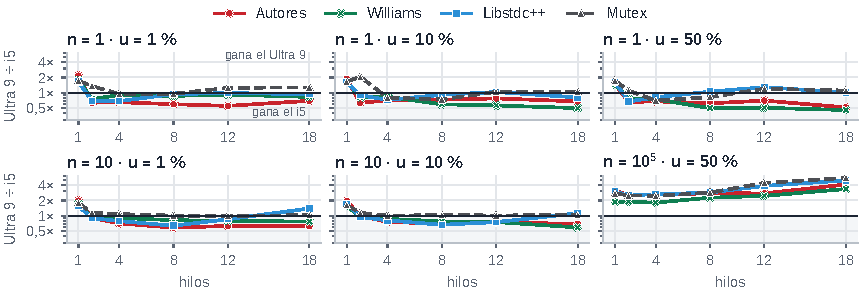
\includegraphics[width=\linewidth]{figuras/s57}
  \vfill\raggedright
  \caja{Autores, una pila y $u = 1$\,\%: con 1 hilo, 44,8\,Mop/s en el i5 y 96,9 en el Ultra 9 (2,2\por); con 12 hilos, 39,1 frente a 21,8 (\textbf{0,56\por}). Sin contención (\pot{5} pilas), el Ultra 9 va 2,7\por{} por delante con 12 hilos.}
  \nota{s57}
\end{frame}

\begin{frame}{Por qué: con contención manda el viaje de la línea, no el núcleo}
  \fuente{matriz\_nucleos.csv y docker/rendimiento.csv (pares); EXPLICACION.md, Partes 5.2 y 6.4}
  \begin{columns}[T]
    \column{0.48\textwidth}
    \porque{el coste de mover una línea}{Con contención, cada operación espera a que la línea compartida llegue desde otro núcleo. El rendimiento lo marca ese viaje, no la velocidad de cálculo.\par\smallskip
    \textbf{Ultra 9:} sus núcleos están lejos entre sí: 47\,ns entre clústeres E y 86\,ns entre núcleos P, medido. Sin fijar los hilos, Linux los reparte entre P y E.\par\smallskip
    \textbf{i5-10400:} un solo bloque de 6 núcleos, y con SMT dos hilos pueden compartir núcleo, con sus cachés L1 y L2: la línea a veces ni se mueve.}
    \column{0.48\textwidth}
    \sub{La misma física, medida en el Ultra 9}\footnotesize
    Dos hilos que comparten L2 rinden casi el doble que cualquier otra pareja:
    \par\smallskip\small
    \begin{tabular}{@{}lr@{}}
      \toprule
      \textbf{Autores, 2 hilos, $n = 1$, $u = 50$\,\%} & \textbf{Mop/s}\\
      \midrule
      Mismo clúster (L2 compartida) & 6,21\\
      Clústeres distintos & 3,41\\
      Dos núcleos P & 3,29\\
      \bottomrule
    \end{tabular}
    \par\medskip
    \aviso{\textbf{Hipótesis}: no se midió la latencia entre núcleos del i5 ni dónde colocó Linux cada hilo. Para confirmarlo: fijar los hilos en el i5 a hermanos de SMT y a núcleos distintos.}
  \end{columns}
  \nota{s58}
\end{frame}

\begin{frame}{Sin contención, más núcleos y más caché sí cuentan}
  \fuente{rendimiento.csv del i5-10400 y del Ultra 9 (correccion), $n = \pot{5}$, $u = 50$\,\%}
  \begin{columns}[T]
    \column{0.46\textwidth}\small\renewcommand{\arraystretch}{1.15}
    \begin{tabular}{@{}lrrrr@{}}
      \toprule
      $n = \pot{5}$ · $u = 50$\,\% & \multicolumn{2}{c}{\textbf{i5-10400}} & \multicolumn{2}{c}{\textbf{Ultra 9}}\\
      \cmidrule(lr){2-3}\cmidrule(l){4-5}
      Mop/s & 12\,h & 18\,h & 12\,h & 18\,h\\
      \midrule
      \alg{cAutores}{Autores} & 26,7 & 24,2 & 73,2 & 98,9\\
      \alg{cLibs}{Libstdc++} & 18,4 & 19,5 & 70,5 & 95,9\\
      \alg{cWilliams}{Williams} & 18,0 & 18,5 & 44,1 & 61,9\\
      \alg{cMutex}{Mutex} & 16,9 & 18,7 & 74,2 & 102,6\\
      \bottomrule
    \end{tabular}
    \column{0.5\textwidth}
    \porque{ya no hay línea disputada}{Con cien mil pilas, dos hilos casi nunca coinciden. Cada uno trabaja en su rincón y el límite pasa a ser cuántos núcleos hay y cuánta memoria cabe cerca. El i5 se estanca al llegar a sus 12 hilos de hardware; el Ultra 9 sigue subiendo hasta 18.}
  \end{columns}
  \vfill
  \caja{En el i5, Autores gana con claridad a los otros tres. En el Ultra 9, Autores, Libstdc++ y Mutex van juntos: la misma tendencia al empate que con \pot{6} pilas y los binarios oficiales.}
  \nota{s59}
\end{frame}

\begin{frame}{Latencia: el mismo orden en las dos máquinas}
  \fuente{latencia.csv del i5-10400 y del Ultra 9 (correccion); 100\,000 muestras, sin el coste del reloj}
  \centering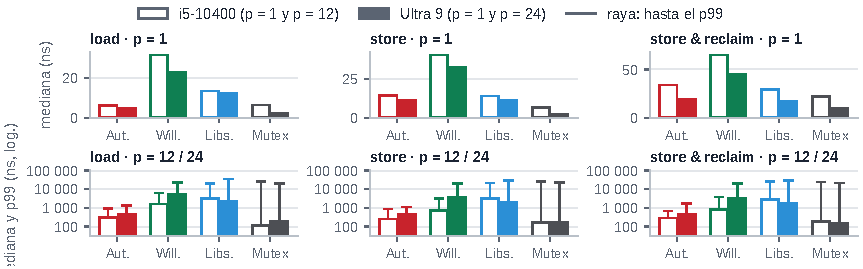
\includegraphics[width=\linewidth]{figuras/s60}
  \vfill\raggedright
  \caja{Sin contención el orden es idéntico: Williams es siempre el más lento. Con contención, la mediana más baja es la del Mutex, pero \textbf{la cola más corta es la de Autores} en las dos: p99 de 0,93\,\textmu s en el i5 y 1,32\,\textmu s en el Ultra 9, frente a 21-26\,\textmu s del Mutex.}
  \nota{s60}
\end{frame}

\begin{frame}{El caso del Mutex: depende de la máquina y de la tanda}
  \fuente{nativo/rendimiento.csv; rendimiento.csv del i5-10400 y del Ultra 9 (correccion); replica/informe/03\_rendimiento.md}
  \centering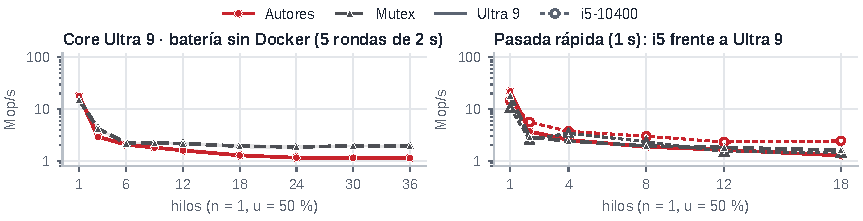
\includegraphics[width=0.86\linewidth]{figuras/s61}
  \par\smallskip\raggedright
  \begin{columns}[T]
    \column{0.49\textwidth}
    \begin{itemize}\footnotesize
      \item \textbf{Ultra 9, batería de 5 rondas:} el Mutex gana desde 3 hasta 36 hilos. Con 24, 1,86 frente a 1,15\,Mop/s.
      \item \textbf{Ultra 9, pasada rápida:} gana desde 8 hilos.
      \item \textbf{i5, pasada rápida:} gana Autores (2,32 frente a 1,51 con 12 hilos); una pasada anterior del equipo daba lo contrario: \textbf{no concluyente}.
    \end{itemize}
    \column{0.47\textwidth}
    \porque{el Mutex duerme a los que esperan}{Si casi todos duermen, la línea casi no viaja. En Autores todos siguen despiertos y sus CAS fallan una y otra vez. Razonable, pero no comprobado.}
  \end{columns}
  \nota{s61}
\end{frame}

\begin{frame}{Qué se concluye de las dos máquinas}
  \fuente{partes 5 y 6 de esta presentación}
  \begin{columns}[T]
    \column{0.48\textwidth}
    {\color{verde}\bfseries Lo que no depende de la máquina}\par\smallskip
    \begin{itemize}\footnotesize
      \item Autores gana a Williams y a Libstdc++ en todos los escenarios con varios hilos.
      \item Libstdc++ se hunde con contención: de 33 a 1,3\,Mop/s en el i5; de 56 a 1,2 en el Ultra 9.
      \item El orden de latencia sin contención, y la cola más corta para Autores con contención.
      \item La corrección: los mismos 0 errores.
    \end{itemize}
    \column{0.48\textwidth}
    {\color{rojo}\bfseries Lo que sí depende}\par\smallskip
    \begin{itemize}\footnotesize
      \item Los Mop/s absolutos, y no en el sentido esperado: con contención gana la máquina «lenta».
      \item Si el Mutex gana a Autores con $n = 1$ y $u = 50$\,\%.
      \item Si los algoritmos empatan sin contención: en el Ultra 9 sí, en el i5 no.
    \end{itemize}
  \end{columns}
  \vfill
  \caja{Lección para leer cualquier benchmark concurrente: \textbf{la velocidad de un núcleo no predice el rendimiento con contención}. Importan la distancia entre núcleos y quién comparte caché.}
  \nota{s62}
\end{frame}
